% Options for packages loaded elsewhere
\PassOptionsToPackage{unicode=true}{hyperref}
\PassOptionsToPackage{hyphens}{url}
%
\documentclass[
  american,
]{article}
\usepackage{lmodern}
\usepackage{amssymb,amsmath}
\usepackage{ifxetex,ifluatex}
\ifnum 0\ifxetex 1\fi\ifluatex 1\fi=0 % if pdftex
  \usepackage[T1]{fontenc}
  \usepackage[utf8]{inputenc}
  \usepackage{textcomp} % provides euro and other symbols
\else % if luatex or xelatex
  \usepackage{unicode-math}
  \defaultfontfeatures{Scale=MatchLowercase}
  \defaultfontfeatures[\rmfamily]{Ligatures=TeX,Scale=1}
\fi
% Use upquote if available, for straight quotes in verbatim environments
\IfFileExists{upquote.sty}{\usepackage{upquote}}{}
\IfFileExists{microtype.sty}{% use microtype if available
  \usepackage[]{microtype}
  \UseMicrotypeSet[protrusion]{basicmath} % disable protrusion for tt fonts
}{}
\makeatletter
\@ifundefined{KOMAClassName}{% if non-KOMA class
  \IfFileExists{parskip.sty}{%
    \usepackage{parskip}
  }{% else
    \setlength{\parindent}{0pt}
    \setlength{\parskip}{6pt plus 2pt minus 1pt}}
}{% if KOMA class
  \KOMAoptions{parskip=half}}
\makeatother
\usepackage{xcolor}
\IfFileExists{xurl.sty}{\usepackage{xurl}}{} % add URL line breaks if available
\IfFileExists{bookmark.sty}{\usepackage{bookmark}}{\usepackage{hyperref}}
\hypersetup{
  pdftitle={mcp: An R Package for Regression With Multiple Change Points},
  pdfauthor={Jonas Kristoffer Lindeløv \^{}\{1*\}},
  hidelinks,
}
\urlstyle{same} % disable monospaced font for URLs
\usepackage[margin=1in]{geometry}
\usepackage{color}
\usepackage{fancyvrb}
\newcommand{\VerbBar}{|}
\newcommand{\VERB}{\Verb[commandchars=\\\{\}]}
\DefineVerbatimEnvironment{Highlighting}{Verbatim}{commandchars=\\\{\}}
% Add ',fontsize=\small' for more characters per line
\usepackage{framed}
\definecolor{shadecolor}{RGB}{248,248,248}
\newenvironment{Shaded}{\begin{snugshade}}{\end{snugshade}}
\newcommand{\AlertTok}[1]{\textcolor[rgb]{0.94,0.16,0.16}{#1}}
\newcommand{\AnnotationTok}[1]{\textcolor[rgb]{0.56,0.35,0.01}{\textbf{\textit{#1}}}}
\newcommand{\AttributeTok}[1]{\textcolor[rgb]{0.77,0.63,0.00}{#1}}
\newcommand{\BaseNTok}[1]{\textcolor[rgb]{0.00,0.00,0.81}{#1}}
\newcommand{\BuiltInTok}[1]{#1}
\newcommand{\CharTok}[1]{\textcolor[rgb]{0.31,0.60,0.02}{#1}}
\newcommand{\CommentTok}[1]{\textcolor[rgb]{0.56,0.35,0.01}{\textit{#1}}}
\newcommand{\CommentVarTok}[1]{\textcolor[rgb]{0.56,0.35,0.01}{\textbf{\textit{#1}}}}
\newcommand{\ConstantTok}[1]{\textcolor[rgb]{0.00,0.00,0.00}{#1}}
\newcommand{\ControlFlowTok}[1]{\textcolor[rgb]{0.13,0.29,0.53}{\textbf{#1}}}
\newcommand{\DataTypeTok}[1]{\textcolor[rgb]{0.13,0.29,0.53}{#1}}
\newcommand{\DecValTok}[1]{\textcolor[rgb]{0.00,0.00,0.81}{#1}}
\newcommand{\DocumentationTok}[1]{\textcolor[rgb]{0.56,0.35,0.01}{\textbf{\textit{#1}}}}
\newcommand{\ErrorTok}[1]{\textcolor[rgb]{0.64,0.00,0.00}{\textbf{#1}}}
\newcommand{\ExtensionTok}[1]{#1}
\newcommand{\FloatTok}[1]{\textcolor[rgb]{0.00,0.00,0.81}{#1}}
\newcommand{\FunctionTok}[1]{\textcolor[rgb]{0.00,0.00,0.00}{#1}}
\newcommand{\ImportTok}[1]{#1}
\newcommand{\InformationTok}[1]{\textcolor[rgb]{0.56,0.35,0.01}{\textbf{\textit{#1}}}}
\newcommand{\KeywordTok}[1]{\textcolor[rgb]{0.13,0.29,0.53}{\textbf{#1}}}
\newcommand{\NormalTok}[1]{#1}
\newcommand{\OperatorTok}[1]{\textcolor[rgb]{0.81,0.36,0.00}{\textbf{#1}}}
\newcommand{\OtherTok}[1]{\textcolor[rgb]{0.56,0.35,0.01}{#1}}
\newcommand{\PreprocessorTok}[1]{\textcolor[rgb]{0.56,0.35,0.01}{\textit{#1}}}
\newcommand{\RegionMarkerTok}[1]{#1}
\newcommand{\SpecialCharTok}[1]{\textcolor[rgb]{0.00,0.00,0.00}{#1}}
\newcommand{\SpecialStringTok}[1]{\textcolor[rgb]{0.31,0.60,0.02}{#1}}
\newcommand{\StringTok}[1]{\textcolor[rgb]{0.31,0.60,0.02}{#1}}
\newcommand{\VariableTok}[1]{\textcolor[rgb]{0.00,0.00,0.00}{#1}}
\newcommand{\VerbatimStringTok}[1]{\textcolor[rgb]{0.31,0.60,0.02}{#1}}
\newcommand{\WarningTok}[1]{\textcolor[rgb]{0.56,0.35,0.01}{\textbf{\textit{#1}}}}
\usepackage{longtable,booktabs}
% Allow footnotes in longtable head/foot
\IfFileExists{footnotehyper.sty}{\usepackage{footnotehyper}}{\usepackage{footnote}}
\makesavenoteenv{longtable}
\usepackage{graphicx,grffile}
\makeatletter
\def\maxwidth{\ifdim\Gin@nat@width>\linewidth\linewidth\else\Gin@nat@width\fi}
\def\maxheight{\ifdim\Gin@nat@height>\textheight\textheight\else\Gin@nat@height\fi}
\makeatother
% Scale images if necessary, so that they will not overflow the page
% margins by default, and it is still possible to overwrite the defaults
% using explicit options in \includegraphics[width, height, ...]{}
\setkeys{Gin}{width=\maxwidth,height=\maxheight,keepaspectratio}
\setlength{\emergencystretch}{3em} % prevent overfull lines
\providecommand{\tightlist}{%
  \setlength{\itemsep}{0pt}\setlength{\parskip}{0pt}}
\setcounter{secnumdepth}{5}
% Redefines (sub)paragraphs to behave more like sections
\ifx\paragraph\undefined\else
  \let\oldparagraph\paragraph
  \renewcommand{\paragraph}[1]{\oldparagraph{#1}\mbox{}}
\fi
\ifx\subparagraph\undefined\else
  \let\oldsubparagraph\subparagraph
  \renewcommand{\subparagraph}[1]{\oldsubparagraph{#1}\mbox{}}
\fi

% Set default figure placement to htbp
\makeatletter
\def\fps@figure{htbp}
\makeatother

\usepackage{amsmath}
\usepackage[utf8]{inputenc}
\usepackage[T1]{fontenc}
\usepackage{setspace}
\onehalfspacing
\newcommand\numberthis{\addtocounter{equation}{1}\tag{\theequation}}
\ifxetex
  % Load polyglossia as late as possible: uses bidi with RTL langages (e.g. Hebrew, Arabic)
  \usepackage{polyglossia}
  \setmainlanguage[variant=american]{english}
\else
  \usepackage[shorthands=off,main=american]{babel}
\fi
\usepackage[]{natbib}
\bibliographystyle{apalike}

\title{mcp: An R Package for Regression With Multiple Change Points}
\author{Jonas Kristoffer Lindeløv \(^{1*}\)}
\date{\(^1\) Department of Communication and Psychology, Aalborg University, Denmark.\break
\(^*\) Corresponding author, Email: \href{mailto:lindeloev@gmail.com}{\nolinkurl{lindeloev@gmail.com}}}

\begin{document}
\maketitle
\begin{abstract}
The R package mcp does flexible and informed Bayesian regression with change points. mcp can infer the location of changes between regression models on means, variances, autocorrelation structure, and any combination of these. Prior and posterior samples and summaries are returned for all parameters and a rich set of plotting options is available. Bayes Factors can be computed via Savage-Dickey density ratio and posterior contrasts. Cross-validation can be used for more general model comparison. mcp ships with sensible defaults, including priors, but the user can override them to get finer control of the models and outputs. The strengths and limitations of mcp are discussed in relation to existing change point packages in R.
\linebreak\linebreak
Keywords: change point, piecewise linear, break point, regression, R, Bayesian
\end{abstract}

\hypertarget{introduction}{%
\section{Introduction}\label{introduction}}

A change point is a location on a dimension where a trend changes. Change point analyses are useful for detecting when a change happens in the rate of accidents due to new policies or practices \citep{raftery1986}, changes in stock prices \citep{chen1997a}, discontinuities in human performance \citep{cowan2000}, and many other scenarios. The widespread applicability of change point analysis is evident from its many names: switch points, break points, broken line, broken stick, (performance) discontinuity models, bilinear regression, piecewise regression, local linear regression, and segmented regression.

More than 10 R packages are available to analyze change points. Most packages detect change points using a threshold on a change-sensitive statistic, including \texttt{ecp} \citep{james2015}, \texttt{bcp} \citep{erdman2007}, \texttt{changepoint} \citep{killick2014}, \texttt{changepoint.np} \citep{haynes2019}, \texttt{TSMCP} \citep{li2018}, \texttt{cpm} \citep{ross2015}, \texttt{EnvCpt} \citep{killick2018}, and \texttt{wbsts} \citep{korkas2018}. This is useful when the number of change points is unknown a priori. Downsides include the fact that the threshold value is somewhat arbitrary and that only point estimates of the change points are returned. Other packages take a fixed number of change points and a user-specified regression model, including \texttt{segmented} \citep{muggeo2008} and \texttt{strucchange::breakpoints()} \citep{zeileis2003}. Downsides to their current implementation include that the same single regression model must apply to all segments.

However, there are many cases where it is desirable to specify the regression model on a per-segment basis. More generally, the analyst often has a priori knowledge about credible coefficient values and the number of change points. For example, human short-term memory capacity can be modeled as a performance discontinuity in accuracy as a function of task difficulty \citep{cowan2000, camos2008, leibovich-raveh2018}. Performance is fast and virtually errorless for easy tasks (a high plateau), but there is an abrupt change to deteriorating accuracy (joined negative slope) when task difficulty exceeds the participant's abilities. Identification of the memory capacity has classically been done by eye-balling graphs or coming up with ad-hoc methods to automate this \citep{leibovich-raveh2018}. Similarly, the effects of many nutrients follow a positive quadratic trend with an exponent between 0 and 1, followed by a plateau at a saturation point \citep{pesti2009}.

In these cases, the number of change points is known, there are a priori bounds on the sign of the coefficients, and all parameters of the model are of interest - not just the change point. There may also be classical regression problems where change points are nuisance effects that need to be co-varied out, so detailed information and tests for \emph{all} parameters (again, not just the change points) can also be useful. \texttt{mcp} aims to fill in these missing pieces in the R landscape. More generally, \texttt{mcp} aims to do regression with multiple change points between user-specified GLMM segments. \texttt{mcp} takes a Bayesian computational approach and, as we shall see, this has the added benefit of properly quantifying uncertainty around the change points - a seemingly impossible task for non-computational methods (\citep{stephens1994, carlin1992}, but see \citep{jensen2013}).

Part 1 of this paper introduces the regression model(s) underlying \texttt{mcp}. Part 2 discusses priors for change point models. Part 3 demonstrates the usage of \texttt{mcp} and it's features. Part 4 discusses the strengths and limitations of \texttt{mcp} in general, and in comparison to the other change point packages in R.

\hypertarget{an-indicator-model-of-multiple-change-points}{%
\section{An indicator model of multiple change points}\label{an-indicator-model-of-multiple-change-points}}

\hypertarget{from-if-else-to-indicators}{%
\subsection{From if-else to indicators}\label{from-if-else-to-indicators}}

Let \(\Delta\) be a location on the dimension of \(x\) where the expectation \(\mu_i\) of the observed \(y_i\) changes from following function \(f_1(\mathbf{x}, \mathbf{\beta_1})\) to \(f_2(\mathbf{x}, \mathbf{\beta_2})\) where \(\mathbf{\beta}\) are regression coefficients. An often-used formalization of a single change point (see e.g.~\citep{stephens1994, carlin1992}) is:

\begin{equation}
\label{eq-ifelse}
\mu_i = \begin{cases}
      f_1(x_i , \mathbf{\beta_1}) & \text{if}\ x_i < \Delta \\
      f_2(x_i , \mathbf{\beta_2}) & \text{if}\ x_i > \Delta \\
    \end{cases}
\end{equation}

For example, a linear segment is \(f_k(x_i , \mathbf{\beta_k}) = \beta_{k, 0} + \beta_{k, 1} \cdot x_i\). One could in principle generalize (\ref{eq-ifelse}) to \(K\) segments (i.e., \(K-1\) change points) by adding more cases and \(\Delta\)s. However, modeling \emph{joined} segments (i.e., where \(\mu\) does not abruptly change at \(\Delta\)) is not straightforward in this formulation. Joining is essential in many change point problems. \texttt{mcp} use a cumulative indicator formulation to achieve this:

\begin{equation}
\label{eq-indicator}
\mu_i = \sum_{k=1}^{K} [x_i > \Delta_{k-1}]  f_k(X_{k, i} , \mathbf{\beta_k})
\end{equation}

where

\begin{equation}
\label{eq-localx}
X_{k,i} = \min\{x_i, \Delta_k\} - \Delta_{k-1}
\end{equation}

The indicator function \([x_i > \Delta_{k-1}]\) evaluates to \(1\) if true and \(0\) if false \citep{knuth1992}. That is, for a given \(x_i\), the parameters of the current and previous segments predict \(\mu_i\) while future segments are multiplied by zero. The indicator must always evaluate to \(1\) for the first segment (\(k = 1\)), which can be achieved by setting \(\Delta_0 = -\infty\). \texttt{mcp} sets \(\Delta_0 = \min(\mathbf{x})\) to achieve the same effect \emph{and} add the constraint that the first change point must occur in the observed range because of the ordering \(\Delta_1 > \Delta_0\).

\(X_{k, i}\) is the ``local'' \(x_i\) to segment \(k\). It is zero at the segment onset (at \(\Delta_{k-1}\)) and plateaus beyond the segment's right boundary (at \(\Delta_k\)). This allows for the modeling of joined segments, handing over \(\mu_i\) like a baton to the next segment. See appendix 2 for the associated likelihood.

\hypertarget{extend}{%
\subsection{Relative, absolute, and segment-specific terms}\label{extend}}

More flexible models can be accommodated by simple manipulations to this basic indicator scheme.

To model \emph{relative} changes in slopes from segment \(k\) to \(k+1\), simply replace \(\beta_{k+1, 1}\) with \(\beta_{k, 1} + \beta_{k + 1, 1}\) so that \(\beta_{k + 1, 1}\) is the \emph{change} in slope. To model \emph{absolute} intercepts in segment \(k + 1\), simply multiply earlier segments with the additional indicator \([x_i < \Delta_k]\) which will evaluate to zero (``turn them off'') when \(x_i\) crosses into segment \(k + 1\).

Various functions can be applied to \(\mathbf{x}\). For example, quadratic trends can be modeled with \(\beta_{k, 2} \cdot X_{k,i}^2\), logarithms with \(\beta_{k, 3} \cdot \log(X_{k,i})\), and so forth for exponents, trigonometric functions, etc.

We can specify per-segment regression models by writing out the sum in (\ref{eq-indicator}) and adding/removing individual terms. For example, (\ref{eq-model}) is a plateau followed by a joined slope followed by a quadratic trend starting at an absolute intercept:

\begin{equation}
\label{eq-model}
\begin{aligned}
X_{2, i} = & \min\{x_i, \Delta_2\} - \Delta_1 \\
X_{3, i} = & \min\{x_i, \Delta_3\} - \Delta_2 \\
\\
\mu_i = & [x_i > \Delta_0] [x_i < \Delta_2] \beta_{1, 0} + && \hspace{2em} \text{Segment 1: intercept} \\
         & [x_i > \Delta_1] [x_i < \Delta_2] \beta_{2, 1} X_{2, i} + && \hspace{2em} \text{Segment 2: slope} \\
         & [x_i > \Delta_2] (\beta_{3, 0} + \beta_{3, 1} X_{3, i}^2) && \hspace{2em} \text{Segment 3: intercept and quadratic}
\end{aligned}
\end{equation}

This model is used as an example throughout this paper. It is visualized in Figure \ref{fig:fitpostprior}.

We can easily share \(\mathbf{\beta}\)s between segments. For example, replacing \(\beta_{3,0}\) with \(\beta_{1,0}\) models identical intercepts in segments 1 and 3 (see Figure \ref{fig:fitpostprior}). Sharing parameters can also be used to model intercept changes while keeping a steady slope between segments.

\hypertarget{generalized-linear-model}{%
\subsection{Generalized linear model}\label{generalized-linear-model}}

Change points can in principle be modeled for all response families and link functions (\(g\)):

\begin{equation}
\label{eq-glm}
\begin{aligned}
y_i & \sim {\rm Normal}(g^{-1}(\mu_i), \sigma) \\
y_i & \sim {\rm Binomial}(n_i, g^{-1}(\mu_i)) \\
y_i & \sim {\rm Poisson}(g^{-1}(\mu_i)) \\
y_i & \sim ...
\end{aligned}
\end{equation}

where \(\sigma\) is the standard deviation of the residuals and \(n_i\) is the number of trials for observation \(y_i\). \texttt{mcp\ 0.3} supports identity (default for \({\rm Normal}\)), log (default for \({\rm Poisson}\)), logit (default for \(\rm{Binomial}\) and \(\rm{Bernoulli}\)), and probit as link functions.

\hypertarget{sigmaar-api}{%
\subsection{Changes in variance and autocorrelation}\label{sigmaar-api}}

Hitherto, we have discussed modeling changes in the central tendency, \(\mu\). Another frequent application is modeling changes in variance. Existing R packages for variance change points models a change from one variance to another, i.e., an intercept change in variance. However, we can model \(\sigma_i\) as a function of \(x_i\) using the same regression model as that for \(\mu_i\) (see \ref{eq-indicator}). As a simple example, this is an absolute change in the mean \emph{and} variance between two segments:

\begin{equation}
\label{eq-variance}
\begin{aligned}
\mu_i = & [x_i > \Delta_0] [x_i < \Delta_1] \beta_{1, 0} + \\
      & [x_i > \Delta_1] \beta_{2, 0} \\
\sigma_i = & [x_i > \Delta_0] [x_i < \Delta_1] \theta_{1, 0} + \\
           & [x_i > \Delta_1] \theta_{2, 0} \\
y_i \sim & {\rm Normal}(\mu_i, \sigma_i)
\end{aligned}
\end{equation}

where, again, \(\Delta_0 = \min(\mathbf{x})\). As with \(\mu\), we can easily model slopes on \(\sigma_i\) as well as periodic (sine and cosine), quadratic, and other functions.

Change point analysis is frequently applied to time-series where the autocorrelation can be modeled using Nth-order autoregressive parameters. In the context of regression, they apply to the residuals on the link scale (\(g(y_i) - \mu_i\)) predicting residual \(i\) as a slope on residual \(i-n\) for each \texttt{n\ =\ 1,\ ...,\ N}:

\begin{equation}
\begin{aligned}
  \epsilon_i & = \sum_{n=1}^{N} \phi_n(g(y_{i-n}) - \mu_{i-n}) \\
  y_i & = {\rm Normal}(\mu_i + \epsilon_i, \sigma_i)
\end{aligned}
\end{equation}

We can subject each \(\phi_n\) to the same regression as we did for \(\mu\) and \(\sigma\), thus identifying the location(s) where the autocorrelation coefficient changes. For AR(N) models, \(\sigma\)s, will represent the \emph{innovations}, i.e., the variance not accounted for by \(\epsilon_i\).

\hypertarget{varying-change-points}{%
\subsection{Varying change points}\label{varying-change-points}}

Each change point parameter (\(\Delta_k\)) can be subjected to regression too. However, this is more involved. Because change points are locations on \(\mathbf{x}\), the preceding and proceeding \(x_i\) (and the associated \(y_i\)) must be observed for all levels of the regressors for the change point to be identifiable. As of v. 0.2.0, \texttt{mcp} supports by-group deviances (``random intercepts'') from the change points (``fixed effects''). \texttt{mcp} implements a hierarchical model where the deviation for group \(k\) from the population-level change point, \(\Delta_k\), is sampled from a normal distribution with mean \(\Delta_k\) and a dispersion parameter \(\varsigma_k\):

\begin{equation}
\delta_{k, j} \sim {\rm Normal}(\Delta_k, \varsigma_k)
\end{equation}

The indicator associated with \(\Delta_k\) in (\ref{eq-indicator}) and (\ref{eq-model}) becomes \([x_i > \delta_{k, j}]\).

While varying effects are often used to ``covary out'' nuisance factors, varying change points are useful for estimating, e.g., individual differences in human memory capacity or other performance discontinuities \citep{lindelov2018}. Modeling the data from all participants in one model increases the precision of the individual parameters over conventional per-participant analyses {[}\citet{leibovich-raveh2018}; kruschke2018{]}.

\hypertarget{segments_api}{%
\subsection{An R formula interface}\label{segments_api}}

R \citep{rcoreteam2019} provides a compact syntax to specify regression models. The coefficients are implicit so that \texttt{y\ \textasciitilde{}\ 1\ +\ x} means \(y_i = \beta_01 + \beta_1x_i\). Python too has begun adopting this syntax via the \texttt{patsy} module.

Given a dataset with the response column \texttt{y} and the predictor column \texttt{x}, you can specify model (\ref{eq-model}) as a list of formulas:

\begin{Shaded}
\begin{Highlighting}[]
\NormalTok{model =}\StringTok{ }\KeywordTok{list}\NormalTok{(}
\NormalTok{  y }\OperatorTok{~}\StringTok{ }\DecValTok{1}\NormalTok{,          }\CommentTok{# Plateau}
    \OperatorTok{~}\StringTok{ }\DecValTok{0} \OperatorTok{+}\StringTok{ }\NormalTok{x,      }\CommentTok{# Joined slope}
    \OperatorTok{~}\StringTok{ }\DecValTok{1} \OperatorTok{+}\StringTok{ }\KeywordTok{I}\NormalTok{(x}\OperatorTok{^}\DecValTok{2}\NormalTok{)  }\CommentTok{# Disjoined quadratic}
\NormalTok{)}
\end{Highlighting}
\end{Shaded}

The coefficients in the three formulas are estimated as are the two change points that define their boundaries. See a fit based on this model in Figure \ref{fig:fitpostprior}.

With \texttt{lme4}, the syntax \texttt{y\ \textasciitilde{}\ (formula\textbar{}group)} was added for varying effects \citep{bates2015}. \texttt{brms} has extended the syntax to model missing values (\texttt{mi(x)}), monotonic effects (\texttt{mo(x)}), and many others \citep{burkner2017}. The \texttt{mcp} model specification builds on this tradition: You can infer changes in the variance using \texttt{sigma(formula)} terms. The following would apply the same regression model to the variance that the model above did for the mean:

\begin{Shaded}
\begin{Highlighting}[]
\NormalTok{model =}\StringTok{ }\KeywordTok{list}\NormalTok{(}
\NormalTok{  y }\OperatorTok{~}\StringTok{ }\DecValTok{1} \OperatorTok{+}\StringTok{ }\KeywordTok{sigma}\NormalTok{(}\DecValTok{1}\NormalTok{),         }\CommentTok{# Plateau in mean and variance}
    \OperatorTok{~}\StringTok{ }\DecValTok{0} \OperatorTok{+}\StringTok{ }\KeywordTok{sigma}\NormalTok{(}\DecValTok{0} \OperatorTok{+}\StringTok{ }\NormalTok{x),     }\CommentTok{# Joined slope}
    \OperatorTok{~}\StringTok{ }\DecValTok{0} \OperatorTok{+}\StringTok{ }\KeywordTok{sigma}\NormalTok{(}\DecValTok{1} \OperatorTok{+}\StringTok{ }\KeywordTok{I}\NormalTok{(x}\OperatorTok{^}\DecValTok{2}\NormalTok{)) }\CommentTok{# Disjoined quadratic}
\NormalTok{)}
\end{Highlighting}
\end{Shaded}

AR(N) takes the format \texttt{ar(order,\ formula)} where \texttt{formula} defaults to an intercept (\texttt{1}). For example, adding \texttt{ar(2)} to a segment would model 2nd order autoregressive residuals for that segment and later segments, until otherwise specified.

The left-hand side of segment 2+ specifies the change point. It defaults to an intercept, i.e., an ``intercept change point''. For example, \texttt{\textasciitilde{}\ x} is interpreted as \texttt{1\ \textasciitilde{}\ x}. You can let a change point intercept vary by a categorical predictor. For example, the following models varying-by-id change points from a plateau to a joined slope where all other parameters are shared:

\begin{Shaded}
\begin{Highlighting}[]
\NormalTok{model =}\StringTok{ }\KeywordTok{list}\NormalTok{(}
\NormalTok{  y }\OperatorTok{~}\StringTok{ }\DecValTok{1}\NormalTok{,              }\CommentTok{# Plateau}
  \DecValTok{1} \OperatorTok{+}\StringTok{ }\NormalTok{(}\DecValTok{1}\OperatorTok{|}\NormalTok{id) }\OperatorTok{~}\StringTok{ }\DecValTok{0} \OperatorTok{+}\StringTok{ }\NormalTok{x  }\CommentTok{# Joined slope at cp_1 + delta_\{1, id\}}
\NormalTok{)}
\end{Highlighting}
\end{Shaded}

These expressions can be combined to characterize a given change point as a change in the mean, variance, autoregression, and varying effect all at once (see an example in Figure \ref{fig:allmodels}).

The response family, the link function, and the prior is specified in the call to \texttt{mcp::mcp()}. For example, the model above can be fitted using Gaussian residuals (the default), Poisson, Binomial, or Bernoulli:

\begin{Shaded}
\begin{Highlighting}[]
\NormalTok{fit_gauss =}\StringTok{ }\KeywordTok{mcp}\NormalTok{(model, data)  }\CommentTok{# Defaults to gaussian(link = "identity")}
\NormalTok{fit_poiss =}\StringTok{ }\KeywordTok{mcp}\NormalTok{(model, data, }\DataTypeTok{family =} \KeywordTok{poisson}\NormalTok{(}\DataTypeTok{link =} \StringTok{"log"}\NormalTok{))}
\end{Highlighting}
\end{Shaded}

Examples of these modeling options are visualized in Figure \ref{fig:allmodels}.

\hypertarget{priors}{%
\section{Priors}\label{priors}}

\hypertarget{default-priors-for-change-points}{%
\subsection{Default priors for change points}\label{default-priors-for-change-points}}

Uninformative priors are assigned to all parameters in the absence of user-provided priors. The default priors should be suitable for estimation in the absence of strong prior knowledge. While setting priors for intercepts, slopes, etc. follow the same principles as other (non-change-point) regression problems, setting priors for the change points presents a challenge of its own. Due to the non-interchangeable segment order in \texttt{mcp}, the prior for the change points should be ordered monotonically in the observed range (\(\min(\mathbf{x}) < \Delta_1 < \Delta_2 < \ldots < \Delta_K < \max(\mathbf{x})\)) while otherwise remaining as uninformative as possible.

The ideal would probably be \protect\hyperlink{dirichlet}{the Dirichlet prior} described below and hence it will be described first. However, it samples 10-100 fold less efficiently than many other priors in \texttt{mcp}, so \texttt{mcp} defaults to using an approximation called \protect\hyperlink{t-tail}{the ``t-tail'' prior}. The Dirichlet and the t-tail prior is visualized for two (\(K = 3\) segments) and five (\(K = 6\)) change points in Figure \ref{fig:defaultpriors}.



\begin{figure}
\includegraphics[width=18.67in]{../mcp/docs/articles/priors_files/figure-html/unnamed-chunk-8-1} \caption{Dirichlet and t-tail priors for two and five change points respectively. Here shown on data where \(\min(\mathbf{x}) = 50\) and \(\max(\mathbf{x}) = 150\). Both priors are flat at \(K = 2\). As \(K\) increase, so does the informativeness of the prior for any given change point.}\label{fig:defaultpriors}
\end{figure}

\hypertarget{dirichlet}{%
\subsubsection{Dirichlet prior}\label{dirichlet}}

\texttt{mcp} supports a scaled and shifted Dirichlet prior on the \emph{difference(s)} between adjacent change points - an approach that is also used to model monotonic effects in brms \citep{burkner2018}. The Dirichlet is itself a simplex: \(\zeta_k > 0\) ensures ordering and while the support is \(\zeta_k \in (0, 1)\) the property that \(\sum_{k=1}^{K-1} \zeta_k = 1\) renders it easy to shift and scale the support to the observed range of \(\mathbf{x}\) (\([\min(\mathbf{x}), \max(\mathbf{x})]\)). Furthermore, the sum of the probability density functions (PDFs) is \({\rm Beta}(1, 1)\), meaning that it represents equal prior credence that a change occurs at any point in the interval \((0, 1)\) before scaling and \([\min(\mathbf{x}), \max(\mathbf{x})]\) after scaling. The absolute location of change point \(\Delta_k\) is the sum of the Dirichlets (differences) of all change points up to - and including - \(k\), i.e., \(\Delta_k = \min(\mathbf{x}) + (\max(\mathbf{x}) - \min(\mathbf{x})) \sum_{j = 1}^k \zeta_k\).

The resulting PDFs for the individual change points are Beta distributions. Specifically, in the default case where all \(\alpha_k = 1\) the marginal change point priors are \(\Delta_k \sim {\rm Beta}(k, K - k)\) after summing but before scaling (see appendix for more details). When there is just one change point, this simplifies to \(\Delta_1 \sim {\rm Beta}(1, 1)\), i.e., a uniform prior in the observed range.

The marginal PDFs for a five-change points model are visualized in figure \ref{fig:defaultpriors}. x-axes are shown for both the unscaled and scaled (to \(\min(\mathbf{x}) = 50\) and \(\max(\mathbf{x}) = 150\)) priors.

\hypertarget{t-tail}{%
\subsubsection{t-tail prior}\label{t-tail}}

For models with one change point, the default prior is simply

\begin{equation}
\Delta_1 \sim {\rm Uniform}(\min(\mathbf{x}), \max(\mathbf{x}))
\end{equation}

which is identical to the Dirichlet prior for one change point. For models with two more change points, a ``t-tail'' prior is the default for all change points. It yields posteriors that are similar to the Dirichlet and is thereby reasonably uninformative. The strength of the t-tail prior is a practical one: it samples much more efficiently.

The t-tail prior is a series of t-distributions where ordering is imposed via left-truncation, i.e., leaving just the tails:

\begin{equation}
\Delta_k \sim t(\mu = 0, \sigma = \frac{1}{K - 1}, \nu = K-2) \hspace{2em} {\rm where} \hspace{2em} 0 < \Delta_1 < ... < \Delta_k < 1
\end{equation}

before scaling. As \(K\) increases, the degrees of freedoms \(\nu\) increase and the variance \(\sigma\) decreases to narrow the priors in a way that keeps the sum of the densities approximately flat (within a factor of two). After shifting to start at \(\min(\mathbf{x})\) and scaling to the range \(\max(\mathbf{x}) - \min(\mathbf{x})\), we get

\begin{equation}
\Delta_k \sim t(\min(\mathbf{x}), \frac{\max(\mathbf{x}) - \min(\mathbf{x})}{K-1}, K-2) \hspace{2em} {\rm where} \hspace{2em} \min(\mathbf{x}) < \Delta_1 < ... < \Delta_k < \max(\mathbf{x})
\end{equation}

While the t-distribution ``base'' is identical for all \(\Delta_k\), the cumulative left-truncation(s) imposes a conditionality that make them differ (see Figure \ref{fig:defaultpriors}). When \(K > 2\), \(\Delta_1\) is a half-t while \(\Delta_{2+}\) are t-tails.

\hypertarget{priors-for-varying-effects}{%
\subsubsection{Priors for varying effects}\label{priors-for-varying-effects}}

The default prior for varying change points are normals that are centered at zero (at the population-level change point) and SD is double the average distance between change points. They are truncated to lie between the two adjacent change points:

\begin{equation}
\delta_{k, j} \sim \mathcal{N}(0, 2 \cdot \frac{\max(\mathbf{x}) - \min(\mathbf{x})}{K - 1}) \hspace{2em} \Delta_{k-1} < \Delta_k + \delta_{k, j} < \Delta_{k + 1}
\end{equation}

\hypertarget{default-priors-for-other-coefficients}{%
\subsection{Default priors for other coefficients}\label{default-priors-for-other-coefficients}}

The default priors for intercepts and slopes in Gaussian families are normals that are vaguely based on data to ensure that they remain uninformative across any order of magnitude. They loosely mimic the priors used in \texttt{brms} \citep{burkner2017}.

For Gaussian families, intercept priors are \(t(0, 3 \cdot {\rm sd}(y), 3)\) slope priors are \(t(0, {\rm sd}(y) / (\max(\mathbf{x}) - \min(\mathbf{x})), 3)\). The prior for \(\sigma_1\)s is \(\mathcal{N}(0, {\rm sd}(y))\) truncated to positive values. A \({\rm Uniform}(-1, 1)\) prior is used on autoregressive coefficients to ensure stationarity \citep{fuller1981}. \(\mathcal{N}(0, 10)\) is used for Poisson intercepts and slopes reflecting an expected value of 1 and a 68.3\% prior credence counts between \(\exp(-10) = 1 / 22026\) and \(\exp(10) = 22026\) and likewise for the total \emph{change} in counts over the observed range of \(\mathbf{x}\). A \(\mathcal{N}(0, 3)\) is used for Bernoulli and binomial intercepts on a logit scale reflecting 68.3\% prior credence in probabilities between 4.7\% and 95.3\%, and \(\mathcal{N}(0, 3 / (\max(\mathbf{x}) - \min(\mathbf{x}))\) for slopes reflecting similar prior credence for the \emph{change} in probabilities over the observed \(\mathbf{x}\).

Additional priors are included for non-default link functions that should be functional for simple models. They are more prone to modeling errors and the user will often need to set appropriate priors on a case-by-case basis. For example, a \texttt{binomial(link\ =\ "identity")} model with a slope can easily result in a binomial rate outside of the allowed interval (\(r \in (0, 1)\)).

\hypertarget{priors_api}{%
\subsection{Setting and using priors}\label{priors_api}}

The naming scheme in \texttt{mcp} is the following: \texttt{cp\_*} are change points (\(\Delta_*\)); \texttt{int\_*} are intercepts (\(\beta_{*, 0}\)); \texttt{{[}var{]}\_*} are slopes (\(\beta{_*, 1}\)). Here \texttt{*} is the segment number (\(k\)).

Users can specify priors using named lists where the values are JAGS code. For example:

\begin{Shaded}
\begin{Highlighting}[]
\NormalTok{prior =}\StringTok{ }\KeywordTok{list}\NormalTok{(}
  \DataTypeTok{cp_1 =} \StringTok{"dunif(10, 50)"}\NormalTok{,      }\CommentTok{# ("Bounded") uniform}
  \DataTypeTok{x_2 =} \StringTok{"dnorm(0, 3) T(0, )"}\NormalTok{,  }\CommentTok{# Positive half-normal}
  \DataTypeTok{int_3 =} \StringTok{"int_1"}              \CommentTok{# Identity}
\NormalTok{)}
\end{Highlighting}
\end{Shaded}

Here, the first change point \texttt{cp\_1} is restricted to the interval \(\Delta_1 \in (10, 50)\) with uniform prior credence in this interval. The slope on \(\mathbf{x}\) in segment 2 (\texttt{x\_2}) is a positive half-normal. The intercept in segment 3 (\texttt{int\_3}) is \emph{shared} with the intercept in segment 1 and they are modeled as one parameter. You can also set constants using e.g., \texttt{int\_3\ =\ 20}, in which case \texttt{int\_3} will not be inferred. The two latter priors are true priors: they express a 100\% belief in the identity and the value respectively.

When no truncation is specified on change points by the user, \texttt{mcp} adds the order restriction (\texttt{T(cp\_i-1,\ MAXX)}). If using the Dirichlet, a priori knowledge about more likely change point locations can be specified by setting \(\alpha_k > 1\) for one or several change points, e.g., \texttt{cp\_2\ =\ "dirichlet(2)"}.

\hypertarget{using-mcp}{%
\section{Using mcp}\label{using-mcp}}

The \href{http://lindeloev.github.io/mcp/}{mcp website} contains numerous worked examples for all \texttt{mcp} features. Here is a simple example, demonstrating a procedure that scales well from simple to complex inference problems.

First, specify a model as a list of formulas. For now, we use \protect\hyperlink{segments_api}{the previously discussed three-segment model}.

\hypertarget{simulate}{%
\subsection{Simulate data}\label{simulate}}

Second, simulate data to evaluate the model's performance. \texttt{mcp} can simulate data for all supported models, including regression on variance and autocorrelation terms. Start by instantiating an \texttt{mcpfit} S3 class without sampling. This object contains all model information, including a \texttt{simulate()} function to simulate data for this model given coefficient values.

Here we simulate 50 data points from some ``true'' parameter values. The simulated data is visualized in figure \ref{fig:fitpostprior}.

\begin{Shaded}
\begin{Highlighting}[]
\CommentTok{# Set up}
\KeywordTok{library}\NormalTok{(mcp)}
\KeywordTok{options}\NormalTok{(}\DataTypeTok{mc.cores =} \DecValTok{3}\NormalTok{)}

\CommentTok{# Get mcpfit object without sampling}
\NormalTok{empty =}\StringTok{ }\KeywordTok{mcp}\NormalTok{(model, }\DataTypeTok{sample =} \OtherTok{FALSE}\NormalTok{)}

\CommentTok{# Simulate data}
\KeywordTok{set.seed}\NormalTok{(}\DecValTok{42}\NormalTok{)}
\NormalTok{df =}\StringTok{ }\KeywordTok{data.frame}\NormalTok{(}\DataTypeTok{x =} \DecValTok{1}\OperatorTok{:}\DecValTok{50}\NormalTok{)  }\CommentTok{# x_i}
\NormalTok{df}\OperatorTok{$}\NormalTok{y =}\StringTok{ }\NormalTok{empty}\OperatorTok{$}\KeywordTok{simulate}\NormalTok{(     }\CommentTok{# associated y_i}
  \DataTypeTok{x =}\NormalTok{ df}\OperatorTok{$}\NormalTok{x,}
  \DataTypeTok{cp_1 =} \DecValTok{12}\NormalTok{, }\DataTypeTok{cp_2 =} \DecValTok{30}\NormalTok{,}
  \DataTypeTok{int_1 =} \DecValTok{5}\NormalTok{, }\DataTypeTok{int_3 =} \DecValTok{5}\NormalTok{,}
  \DataTypeTok{x_2 =} \FloatTok{0.5}\NormalTok{, }\DataTypeTok{x_3_E2 =} \FloatTok{-0.005}\NormalTok{,}
  \DataTypeTok{sigma_1 =} \DecValTok{2}
\NormalTok{)}
\end{Highlighting}
\end{Shaded}

\hypertarget{set-priors-and-inspect-the-prior-predictive}{%
\subsection{Set priors and inspect the prior predictive}\label{set-priors-and-inspect-the-prior-predictive}}

Using the priors discussed in \protect\hyperlink{priors_api}{``Setting and using priors''}, we can sample the prior and do a prior predictive check that the priors jointly cover a reasonable region - not too narrow and not too wide \citep{conn2018} (see figure \ref{fig:fitpostprior}).

\begin{Shaded}
\begin{Highlighting}[]
\NormalTok{fit_prior =}\StringTok{ }\KeywordTok{mcp}\NormalTok{(model, }\DataTypeTok{data =}\NormalTok{ df, }\DataTypeTok{prior =}\NormalTok{ prior, }\DataTypeTok{sample =} \StringTok{"prior"}\NormalTok{)}
\KeywordTok{print}\NormalTok{(fit_prior}\OperatorTok{$}\NormalTok{prior)  }\CommentTok{# Show JAGS code for priors}
\KeywordTok{plot}\NormalTok{(fit_prior)         }\CommentTok{# Prior predictive check}
\end{Highlighting}
\end{Shaded}

\includegraphics{mcp-paper_files/figure-latex/unnamed-chunk-7-1.pdf}

\hypertarget{results-and-interpretation}{%
\subsection{Results and interpretation}\label{results-and-interpretation}}

When you are satisfied with your model and priors, fit it to the simulated data to learn whether the parameters can be recovered. For the present example, we instruct \texttt{mcp()} to sample both the prior and the posterior (\texttt{sample\ =\ "both"}) because we will need the prior to compute a Savage-Dickey Density Ratio later. \texttt{mcp()} defaults to sampling the posterior only.

\begin{Shaded}
\begin{Highlighting}[]
\NormalTok{fit =}\StringTok{ }\KeywordTok{mcp}\NormalTok{(model, }\DataTypeTok{data =}\NormalTok{ df, }\DataTypeTok{prior =}\NormalTok{ prior, }\DataTypeTok{sample =} \StringTok{"both"}\NormalTok{)}
\end{Highlighting}
\end{Shaded}

The \texttt{plot()} function visualizes the inferred model (see Figure \ref{fig:fitpostprior}. Fitted (\texttt{q\_fit}) and/or predictive (\texttt{q\_predict}) quantiles of the highest-density region can be added as well.



\begin{Shaded}
\begin{Highlighting}[]
\KeywordTok{plot}\NormalTok{(fit, }\DataTypeTok{q_fit =} \OtherTok{TRUE}\NormalTok{) }\OperatorTok{+}\StringTok{ }
\StringTok{  }\NormalTok{ggplot2}\OperatorTok{::}\KeywordTok{ggtitle}\NormalTok{(}\StringTok{"Posterior fit"}\NormalTok{) }\OperatorTok{+}
\StringTok{  }
\KeywordTok{plot}\NormalTok{(fit_prior, }\DataTypeTok{lines =} \DecValTok{0}\NormalTok{, }\DataTypeTok{prior =} \OtherTok{TRUE}\NormalTok{, }\DataTypeTok{q_predict =} \KeywordTok{c}\NormalTok{(}\FloatTok{0.2}\NormalTok{, }\FloatTok{0.8}\NormalTok{)) }\OperatorTok{+}\StringTok{ }
\StringTok{  }\NormalTok{ggplot2}\OperatorTok{::}\KeywordTok{ggtitle}\NormalTok{(}\StringTok{"Prior predictive"}\NormalTok{)}
\end{Highlighting}
\end{Shaded}

\begin{figure}
\centering
\includegraphics{mcp-paper_files/figure-latex/fitpostprior-1.pdf}
\caption{\label{fig:fitpostprior}Prior predictive and posterior fits from the model discussed in the main text and presented in equation (\ref{eq-model}). \textbf{Left:} Raw data (black dots, simulated in the main text) with 25 draws from the joint posterior (grey lines) and 95\% highest density interval (dashed red lines). Posterior distributions of the change points are shown in blue - one line for each chain. \textbf{Right:} The same as left, but for prior samples and with a 60\% prediction interval (green lines). Note that the uniform prior on the first change point was set manually in \protect\hyperlink{priors_api}{the section on the prior API} and is not an mcp default.}
\end{figure}

\texttt{summary()} summarises the posterior means and the highest density intervals for each parameter. When the data are simulated, the values used for simulation are included as well to ease model evaluation (columns \texttt{sim} and \texttt{match} which is ``OK'' if \texttt{lower\ \textless{}\ sim\ \textless{}\ upper}). We see that all parameters were well recovered in this case. The summary includes diagnostics of the MCMC sampling as well. A Gelman-Rubin convergence diagnostic below 1.1 is conventionally taken as an indication that the MCMC chains have converged well \citep{gelman1992}. The effective sample size expresses the amount of information that the MCMC chains carry for each parameter \citep{martino2017}. It is inversely related to the MCMC autocorrelation. These diagnostics are computed using the \texttt{coda} package \citep{plummer2006}. The model performs appropriately on all accounts here.

\begin{Shaded}
\begin{Highlighting}[]
\KeywordTok{summary}\NormalTok{(fit)}
\end{Highlighting}
\end{Shaded}

\begin{verbatim}
## Family: gaussian(link = 'identity')
## Iterations: 9000 from 3 chains.
## Segments:
##   1: y ~ 1
##   2: y ~ 1 ~ 0 + x
##   3: y ~ 1 ~ 1 + I(x^2)
## 
## Population-level parameters:
##     name match    sim    mean  lower   upper Rhat n.eff
##     cp_1    OK 12.000 16.6791 11.734 21.0828  1.0   590
##     cp_2       30.000 29.4474 29.000 29.9631  1.1   329
##    int_1    OK  5.000  5.5093  4.606  6.4882  1.0  1547
##    int_3    OK  5.000  5.5093  4.606  6.4882  1.0  1547
##  sigma_1    OK  2.000  2.3394  1.886  2.8310  1.0  3869
##      x_2    OK  0.500  0.7123  0.343  1.0916  1.0   684
##   x_3_E2    OK -0.005 -0.0072 -0.014 -0.0014  1.0  2284
\end{verbatim}

While \texttt{plot()} visualizes the whole model, \texttt{plot\_pars()} visualizes individual parameters. The default plot includes a posterior density overlay with one curve for each chain, and a trace plot to inspect convergence history and mixing. Under the hood, this leverages the \texttt{bayesplot} package \citep{gabry2019} and supports many different plot types.

Notice that the change point posteriors do not conform to any readily known distribution, highlighting the need for a computation approach. This propagates to parameters of the following segment(s) as can be seen in the joint distribution between the change point to the second segment (\texttt{cp\_1}) and its slope (\texttt{x\_2}) (see Figure \ref{fig:pars}).

\begin{Shaded}
\begin{Highlighting}[]
\KeywordTok{plot_pars}\NormalTok{(fit, }\DataTypeTok{pars =} \KeywordTok{c}\NormalTok{(}\StringTok{"cp_1"}\NormalTok{, }\StringTok{"cp_2"}\NormalTok{, }\StringTok{"x_2"}\NormalTok{)) }\OperatorTok{+}\StringTok{ }
\StringTok{  }\KeywordTok{plot_pars}\NormalTok{(fit, }\DataTypeTok{pars =} \KeywordTok{c}\NormalTok{(}\StringTok{"cp_1"}\NormalTok{, }\StringTok{"x_2"}\NormalTok{), }\DataTypeTok{type =} \StringTok{"hex"}\NormalTok{)}
\end{Highlighting}
\end{Shaded}

\begin{figure}
\includegraphics[width=1\linewidth]{mcp-paper_files/figure-latex/pars-1} \caption{\textbf{Left:} Posteriors and trace plots for selected parameters (rows) and three chains (colors) of the model from the main text (see also Figure \ref{fig:fitpostprior}). The mixing and convergence is satisfactory here, as also indicated in the output from \texttt{summary()} discussed in the main text. \textbf{Right:} A joint density plot for the first change point and the slope in the following segment. These plots are the output of \texttt{plot\_pars()}. Note that these posteriors were also plotted in Figure \ref{fig:fitpostprior}. The change point posteriors rarely conform to well-known distributions.}\label{fig:pars}
\end{figure}



\hypertarget{testing-parameter-values}{%
\subsection{Testing parameter values}\label{testing-parameter-values}}

Hypotheses about parameter values can be tested with the \texttt{hypothesis()} function which is heavily inspired by \texttt{brms::hypothesis()} \citep{burkner2017}.

The Savage-Dickey density ratio is the ratio of the prior and posterior density at a particular value and corresponds to a point Bayes Factor \citep{verdinelli1995}. Point Bayes Factors are as much an expression of the prior as the posterior, so careful specification of the prior is warranted.

In the current example, we may want to test whether \(x_2 = 0.5\), i.e., corresponding to a one-sample t-test. The output includes a parameter estimate of the deviance from the hypothesis. It also includes \texttt{p} and \texttt{BF} will express the evidence \emph{in favor} of the specified hypothesis. The inverse (i.e., \(1 - p\) and \(1 / BF\)) is the evidence in favor of the alternative. The Savage-Dickey test yields around \(BF = 5\) strengthening the belief in this point hypothesis by a factor of around 6 relative to the prior belief. Note that \texttt{mcp} is currently the only R package that can quantify evidence \emph{for} a null hypothesis. Frequentist analyses assume the null hypothesis and hence cannot (directly) estimate it's credibility \citep{kruschke2018, colquhoun2014}.

Directional hypotheses operate entirely on the posterior, comparing the proportion of posterior density (number of MCMC samples) above or below a particular value. This can be exploited to test interval hypotheses like ROPE \citep{kruschke2011}, e.g., whether \(x\_2 \in (0.2, 0.8)\). Here, the Bayes Factor is around \(BF = 2.5\).

Hypotheses can also concern relationships between parameters, e.g., akin to two-sample t-tests. For example, we can test whether \(\Delta_1 < \Delta_2 / 2\). The evidence seems to favor the alternative hypothesis by a factor of around \(1 / 0.25 = 4\).

Since the values of the model's 7 parameters were inferred from just 50 data points, the likelihoods (and hence the posteriors) are relatively wide. They will narrow with larger sample sizes resulting in more extreme probabilities and Bayes Factors.

\begin{Shaded}
\begin{Highlighting}[]
\KeywordTok{hypothesis}\NormalTok{(fit, }\KeywordTok{c}\NormalTok{(}\StringTok{"x_2 = 0.5"}\NormalTok{, }
                  \StringTok{"x_2 > 0.2 & x_2 < 0.8"}\NormalTok{,}
                  \StringTok{"cp_1 < cp_2 / 2"}\NormalTok{))}
\end{Highlighting}
\end{Shaded}

\begin{verbatim}
##              hypothesis mean lower upper    p   BF
## 1         x_2 - 0.5 = 0 0.21 -0.16  0.59 0.84 5.41
## 2 x_2 > 0.2 & x_2 < 0.8   NA    NA    NA 0.70 2.37
## 3   cp_1 - cp_2 / 2 < 0 1.96 -3.18  6.23 0.20 0.25
\end{verbatim}

\hypertarget{model-comparison}{%
\subsection{Model comparison}\label{model-comparison}}

\texttt{mcp} supports model comparison via cross-validation via the \texttt{loo} package \citep{vehtari2017}, i.e., by comparing the out-of-sample predictive accuracy of models. Continuing our example, we can test the very existence of the first change point by comparing it to a null model where the first two segments are collapsed into one linear segment.

Briefly, \texttt{loo} sums the log-density of the posterior predictive density at one data point when the model is fitted on the remaining data points. This is repeated for all data points and averaged. Doing this, the Estimated Log-Predictive Density (ELPD) indicates how much credence the model ascribes to out-of-sample data and hence is a relative index of its predictive performance. One would favor a model to the degree that it has superior predictive performance (greater ELPD) and the column \texttt{elpd\_diff} shows this difference \citep{vehtari2017, gelman2013b}. Like any model comparison approach, Bayesian cross-validation is often useful but there are (edge) cases where the predictive performance of a model is underestimated \citep{gronau2019a}. Hopefully, future versions of \texttt{mcp} will include more options for model comparison, e.g., via the \texttt{bridgesampling} package \citep{gronau2018}, so that convergence between multiple methods can bolster inferential conclusions.

Here, the existence of the change point is favored over the null model but only weakly. As with the parameter-level hypotheses discussed previously, the out-of-sample predictive performance of the models will be better discriminable as the sample size increases.

\begin{Shaded}
\begin{Highlighting}[]
\CommentTok{# Define the null model}
\NormalTok{model_null =}\StringTok{ }\KeywordTok{list}\NormalTok{(}
\NormalTok{  y }\OperatorTok{~}\StringTok{ }\DecValTok{1} \OperatorTok{+}\StringTok{ }\NormalTok{x,      }\CommentTok{# One linear segment}
    \OperatorTok{~}\StringTok{ }\DecValTok{1} \OperatorTok{+}\StringTok{ }\KeywordTok{I}\NormalTok{(x}\OperatorTok{^}\DecValTok{2}\NormalTok{)  }\CommentTok{# Disjoined quadratic}
\NormalTok{)}
\NormalTok{prior =}\StringTok{ }\KeywordTok{list}\NormalTok{(}\DataTypeTok{x_1 =} \StringTok{"dnorm(0, 3) T(0, )"}\NormalTok{, }\DataTypeTok{int_2 =} \StringTok{"int_1"}\NormalTok{)  }\CommentTok{# Same prior}

\CommentTok{# Sample it}
\NormalTok{fit_null =}\StringTok{ }\KeywordTok{mcp}\NormalTok{(model_null, }\DataTypeTok{data =}\NormalTok{ df, }\DataTypeTok{prior =}\NormalTok{ prior)}
\end{Highlighting}
\end{Shaded}

\begin{Shaded}
\begin{Highlighting}[]
\CommentTok{# Compute loos and compare}
\NormalTok{fit}\OperatorTok{$}\NormalTok{loo =}\StringTok{ }\KeywordTok{loo}\NormalTok{(fit)}
\NormalTok{fit_null}\OperatorTok{$}\NormalTok{loo =}\StringTok{ }\KeywordTok{loo}\NormalTok{(fit_null)}
\NormalTok{loo}\OperatorTok{::}\KeywordTok{loo_compare}\NormalTok{(fit}\OperatorTok{$}\NormalTok{loo, fit_null}\OperatorTok{$}\NormalTok{loo)  }\CommentTok{# Can take more loos}
\end{Highlighting}
\end{Shaded}

\begin{verbatim}
##        elpd_diff se_diff
## model1  0.0       0.0   
## model2 -0.9       4.3
\end{verbatim}

\hypertarget{apply-to-real-data}{%
\subsection{Apply to real data}\label{apply-to-real-data}}

The previous steps served to crystallize an analysis plan. For confirmatory research, it is recommended to pre-register the analysis plan and the associated code at this point \citep{munafo2017}. Running the analysis with observed data is then merely a matter of ``plugging it in'' and running the analyses.



\begin{figure}
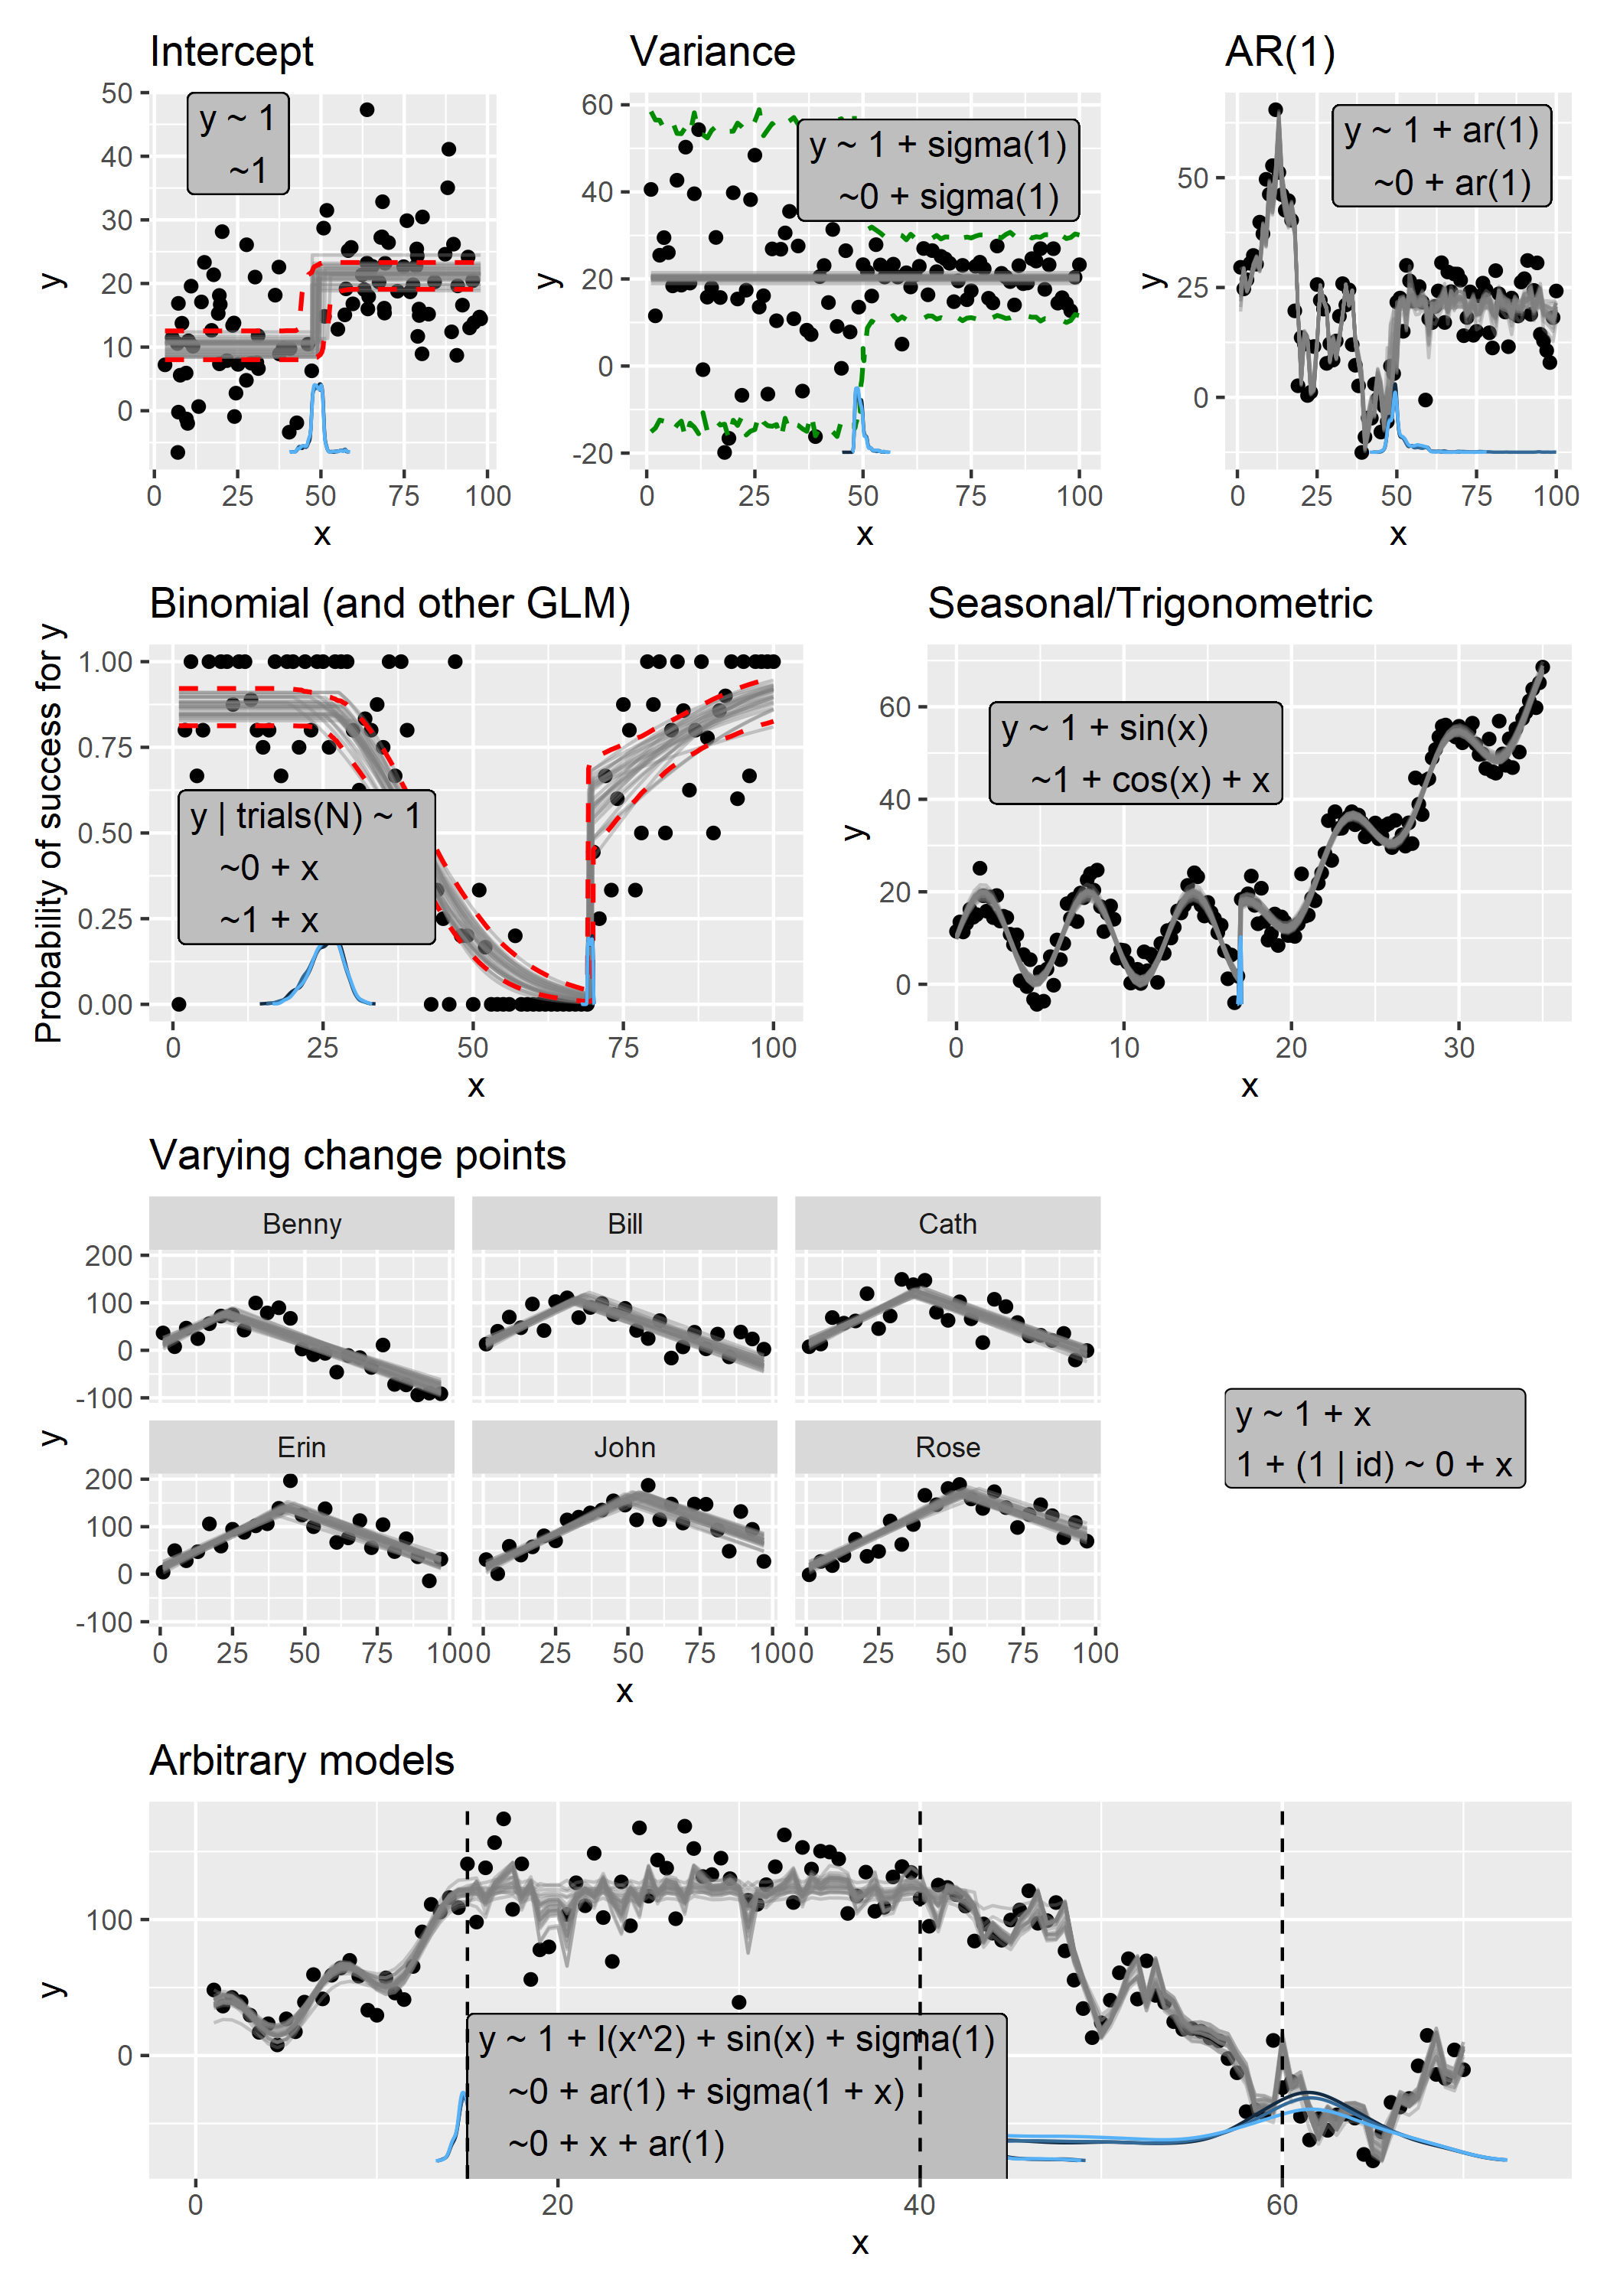
\includegraphics[width=5.6in]{all_plots} \caption{Some example mcp models with data (black dots), 25 posterior draws (grey lines), change point posteriors (blue densities), 95\% fit intervals (red dashed lines), and 95\% prediction intervals (green dashed lines). All plots were made with \texttt{plot()} and the data was simulated using the \texttt{simulate()} function. Other capabilities of \texttt{mcp}, not shown here, include Poisson regression and regression on \texttt{sigma()}/\texttt{ar()} (\protect\hyperlink{sigmaar-api}{see the section on modeling variance}).}\label{fig:allmodels}
\end{figure}

\hypertarget{compare_packages}{%
\section{Strengths and limitations}\label{compare_packages}}

\hypertarget{inferring-change-points-and-a-warning-about-intervals}{%
\subsection{Inferring change points and a warning about intervals}\label{inferring-change-points-and-a-warning-about-intervals}}

\texttt{mcp} uses JAGS \citep{plummer2003} for inference. This is a notable difference to other packages. Multiple change point problems with unknown parameters are analytically intractable (\citep{stephens1994, carlin1992}, but see \citep{jensen2013}). Therefore, change points are typically inferred using variations over two types of search algorithms:

\begin{itemize}
\item
  User-specified number of change points: iterate over possible locations of the \(K-1\) change points and return the fit that minimizes the cost of the \(K\) regression models.
\item
  An unknown number of change points: Compute a statistic that is sensitive to changes. Return a change point every time the statistic passes a threshold. CUSUM \citep{page1954, lee2003} is one such an algorithm that is sensitive to changes in the intercept.
\end{itemize}

These procedures are practical and fast. However, their procedural nature also means that the statistical properties of the inferred change points are unknown and hence confidence intervals cannot readily be computed. One exception is the \texttt{segmented} package which implements a score-based confidence interval \citep{muggeo2017}. Care should be taken not to interpret frequentist intervals as a Bayesian posterior. The posteriors are often multi-modal and asymmetric (see e.g.~Figure \ref{fig:pars}, Figure \ref{fig:allmodels} and \citep{raftery1986}). Therefore, simple intervals (whether frequentist or Bayesian) do not necessarily represent credible change point locations.

Change points can be inferred using a Gibbs sampler (and later optimizations) in the absence of an analytical solution \citep{stephens1994, carlin1992}. Since the advent of the BUGS language for Gibbs samplers in the 1990s \citep{lunn2012}, Gibbs samplers have been used to identify change points in Generalized Linear Mixed Models (GLMM) and Time Series, among many others. I refer to\citep{stephens1994, carlin1992} for a detailed exposition of how Gibbs samplers infer change points.

\texttt{mcp} uses JAGS \citep{plummer2003} but is built with an abstraction layer that represents the model in a sampler-agnostic way so that other samplers can easily be supported in the future. JAGS was chosen for the initial versions of \texttt{mcp} because (1) model compilation is fast so total run time is often lower than \texttt{stan}, (2) the install procedure is similar across operating systems, (3) and the JAGS code is highly similar to R code, making it easier for R users to inspect and learn. \texttt{stan} \citep{carpenter2017} may be supported in the future since it is faster once the model has compiled. \texttt{stan} is also expected to be superior for large datasets, complex models, and the Dirichlet prior.

\hypertarget{strengths}{%
\subsection{Strengths}\label{strengths}}

The mcp website contains \href{https://lindeloev.github.io/mcp/articles/packages.html}{a detailed comparison of R packages for multiple change point analysis}, including \texttt{mcp}, \texttt{segmented} \citep{muggeo2008}, \texttt{strucchange} \citep[\citet{zeileis2003}]{zeileis2002}, \texttt{ecp} \citep{james2015}, \texttt{bcp} \citep{erdman2007}, \texttt{changepoint} \citep{killick2014}, \texttt{changepoint.np} \citep{haynes2019}, \texttt{TSMCP} \citep{li2018}, \texttt{cpm} \citep{ross2015}, \texttt{EnvCpt} \citep{killick2018}, \texttt{wbsts} \citep{korkas2018}, and others.

To the best of my knowledge, \texttt{mcp} is unique in the following ways:

\begin{itemize}
\item
  \textbf{Modeling:} (1) \texttt{mcp} supports a larger number of regression models while most packages model either (joined) slope changes or intercept-only changes. (2) mcp allows regression models to differ between segments while other packages assume identical segment structures. (3) \texttt{mcp} can model varying change points and detect changes in autoregression. (4) \texttt{mcp} can do regression on \(\sigma\) (variance) and \(\psi\) (autocorrelation) for change point problems.
\item
  \textbf{Output:} (1) \texttt{mcp} computes posteriors for the change points (and other parameters), overcoming the problems with interval estimates for change point problems. (2) \texttt{mcp} can simulate data for all these models and directly assess parameter recovery. (3) \texttt{mcp} provides many plot options and returns the plots as \texttt{ggplot2} objects so that the user can customize the plots further.
\item
  \textbf{Inference:} (1) \texttt{mcp} can include prior knowledge about individual parameters, model constant and identical coefficients (e.g., shared between segments). (2) \texttt{mcp} can do point-, directional-, and interval-tests on individual parameters. Because of this modeling flexibility, a greater number of models can be compared.
\end{itemize}

Taken together, we may say that the strength of \texttt{mcp} is for \emph{informed} analysis, i.e., when prior knowledge can be flexibly incorporated as specific model(s) or prior distributions on parameters.

When applying all change point packages to a simple three-intercept problem, half of the packages found the two change points without quantifying uncertainty (\texttt{EnvCpt}, \texttt{strucchange::breakpoints}, \texttt{cpm}, \texttt{changepoint.np}, and \texttt{ecp::e.divisive}), while the other half did not recover them (\texttt{segmented}, \texttt{changepoint}, most methods in \texttt{ecp}, \texttt{TSMCP}, and \texttt{wbsts}).

\texttt{mcp} aims to be user-friendly. It includes more than 100 stop conditions with helpful error messages. For example, if JAGS throws an error (e.g., when the user-provided prior results in a directed cycle), this error is returned along with an empty \texttt{mcpfit} object containing the model code so that it can be inspected by the user. The test suite for \texttt{mcp} currently includes more than 1.700 tests that cover 88\% of the code, reducing the chance that the end-user encounters a bug.

The source code is hosted on GitHub. It is less than 2.000 lines making \texttt{mcp} relatively lightweight to maintain, extend, and collaborate on.

\hypertarget{limitations}{%
\subsection{Limitations}\label{limitations}}

Where \texttt{mcp} falls short, I find that \texttt{segmented}, \texttt{EnvCpt}, and \texttt{bcp} are recommendable packages provided that the data conforms to the smaller range of models supported by these packages.

\texttt{mcp} cannot detect the number of change points in a dataset. \texttt{mcp} can use \texttt{loo} to compare N models, e.g., with \(K = 1, 2, \ldots, N\) segments but this grows intractable for large \(K\).

Due to the order-restriction of the change point priors in \texttt{mcp}, each prior quickly becomes highly localized for larger \(K\). Specifically, the posteriors may ``shrink'' towards these priors in undesirable ways if the data set is not large enough that the likelihood will dominate the prior, e.g., \(K = 10\) for 100 data points. While \texttt{mcp} quantifies the credence that a \emph{given} change point occurs at \(x_i\), questions for large \(K\) may better be posed as the credence that \emph{any} change point occurs at \(x_i\).

\texttt{mcp} is the slowest of the reviewed packages and may be too computationally heavy for time-critical analyses of large datasets, e.g., 100.000 data points. To speed up inference, \texttt{mcp} supports parallel processing via the \texttt{future} and \texttt{future.apply} packages \citep{bengtsson2019}. Furthermore, fewer posterior samples are likely needed for large datasets.

Lastly, \texttt{mcp} does not currently model multivariate data (\texttt{ecp}, \texttt{bcp}, or \texttt{TSMCP} are recommended). Furthermore, \texttt{mcp} does not currently support survival models, Moving-Average/ARIMA autocorrelation, or more than one predictor variable. \texttt{segmented} may be superior in these respects.

\hypertarget{conclusion}{%
\section{Conclusion}\label{conclusion}}

\texttt{mcp} aims to fill in a missing piece in the change point world: flexible per-segment regression models with rich inference information. In concert with the packages doing automatic detection of the number of change points, along with more efficient (but also more limited) packages for a known number of change points, R users now have a great plethora of options that should cover most needs.

\hypertarget{appendix}{%
\section{Appendix}\label{appendix}}

\hypertarget{marginal-dirichlet-priors}{%
\subsection{Marginal Dirichlet Priors}\label{marginal-dirichlet-priors}}

Before shifting and scaling, the prior for change point \(k\) of total \(K-1\) change points will correspond to:

\begin{equation}
\Delta_k \sim {\rm Beta}(\sum_{z = 1}^k \alpha_z, \sum_{z=k}^{K-1} \alpha_z)
\end{equation}

When all \(\mathbf{\alpha} = 1\), this simplifies to:

\begin{equation}
\Delta_k \sim {\rm Beta}(k, K - k)
\end{equation}

\hypertarget{the-likelihood-for-a-multiple-change-point-model}{%
\subsection{The Likelihood for a multiple change point model}\label{the-likelihood-for-a-multiple-change-point-model}}

Generalizing equation (\ref{eq-indicator}) from Carlin et al.~(1992) to multiple change points and inserting (\ref{eq-indicator}) and (\ref{eq-localx}), we get the likelihood:

\begin{equation}
\begin{aligned}
\mathcal{L}(\mathbf{y}) & = \prod_{k = 1}^K\prod_{i = \Delta_{k-1}}^{\Delta_k} [x_i > \Delta_{k-1}]\cdot P_k(X_{k, i}, \mathbf{\beta_k}) \\
                        & = \prod_{k = 1}^K\prod_{i = \Delta_{k-1}}^{\Delta_k} [x_i > \Delta_{k-1}]\cdot P_k(\max\{x_i, \Delta_{k+1}\} - \Delta_k, \mathbf{\beta_k})
\end{aligned}
\end{equation}

where \(P_k\) is the density associated with \(f_k\) and the family in question (e.g., Gaussian or Binomial). An additional indicator is needed to model absolute intercepts, as discussed in section \ref{#extend}.

\renewcommand\refname{References}
  \bibliography{mcp-paper}

\end{document}
